\subsection{Objectives of the \sDIPC\ subproject}
\label{sec.obj.dipc}

DIPC takes three major roles in this project: {\bf i:} coordinates the integration, commissioning and operation of \Next\ (in collaboration with IFIC); 
{\bf ii:} hosts and participates in the construction, commissioning and operation of the \HDEMO\ prototype, and 
{\bf iii:} co-coordinates \NHD\ integration (in collaboration with IFIC and LSC). 

   
\subsubsection*{Integration, coordination and operation of \Next}

\indent

%\begin{figure}[!htb]
%\centering
%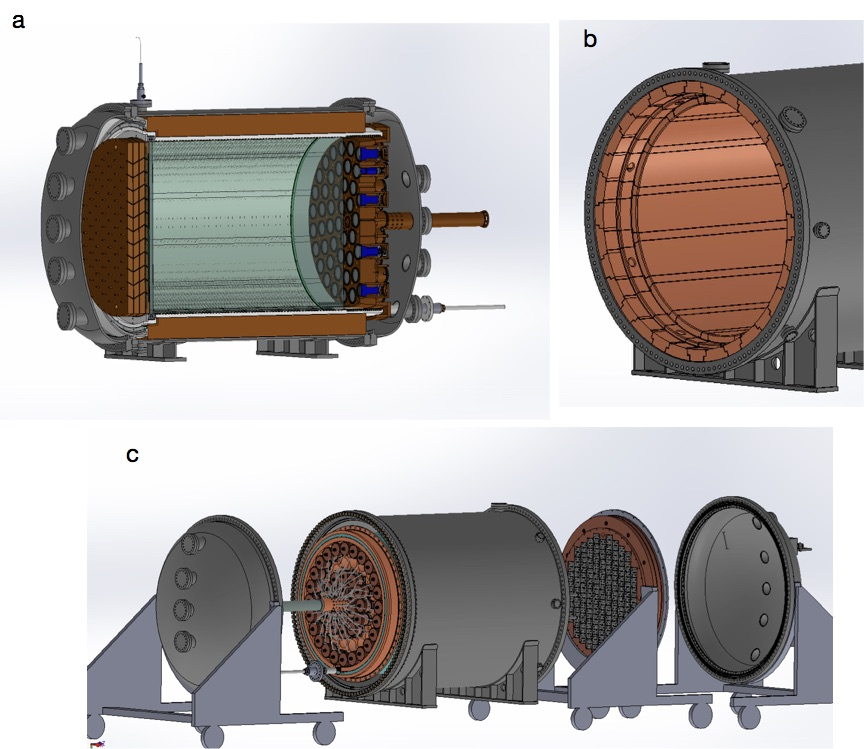
\includegraphics[width=0.7\textwidth]{img2/Next100Collage.jpg}
%\caption{\small a) The NEXT-100 apparatus; b) a detail showing the ICS inside the pressure vessel; c) a detail showing the integration of the detector. ICS comes first, then field cage is slid in, then the end-caps carrying the heavy copper supports for the tracking plane and energy plane are moved in.} 
%\label{fig.n100e}
%\end{figure} 
%

Integration of \Next\ components will proceed during the first half of 2022. The integration task, in which all the subsystems (EP, TP, TPC and ICS) are assembled inside the \Next\ PV and the full detector is placed inside the lead castle (figure \ref{fig.n100e}), will be coordinated by the DIPC, and involves directly the Technical Coordinator (TC), two senior engineers who serve as Integration Managers ({\bf IMs}) and the {\bf GLIMOS}, who is an expert in safety and links with the LSC personnel. The TC, the GLIMOS and one of the IMs are personnel from DIPC, while the second IM is from IFIC. 

The commissioning and operation of the system will occur during the second half of 2022 and involves the Run Coordinator ({\bf RC}), who has the following crucial functions: 


\indent

\begin{itemize}[noitemsep,topsep=0pt,parsep=0pt,partopsep=0pt]
\item {\bf Monitor the day-by-day operation of the detector}, ensuring that safety protocols are met and operation parameters are respected. This includes the status of the gas system, the high voltages, and the sensors's voltage. All those systems are followed by slow-controls which can react automatically to emergencies such as over pressure ---that situation would trigger an automatic gas recovery---, voltage excursions ---which would result in an automatic voltage shutdown--- etc. Nevertheless, the status of the detector must be assessed every day, to guarantee safe and stable operations in the long term and correct any potential problem, such as leaks, broken channels etc. DIPC coordinated the operation of \NEW, acquiring invaluable experience during the 5 years-long run. 
 
\item {\bf Monitor physics parameters},  in particular the electron lifetime, who has a major impact in the energy resolution. Again, the experience of \NEW\ will be important here. The initial electron lifetime of the former detector was \SI{100}{\micro\second}, to be compared with the lifetime in the physics runs, in excess of 
\SI{10}{\milli\second}, \emph{i.e.}, an improvement of two orders of magnitude, which was achieved as we developed the know-how on the technology. 

\item {\bf Organise the shifts}, both in-person (scientists and engineers present at the LSC) and remote (scientists following on-line the detector evolution). The RC organises weekly run-coordination meetings where all the aspects of detector's operation are discussed. 
\end{itemize}

\indent

\subsubsection*{\HDEMO\ prototype}

\indent

The \HDEMO\ prototype will be hosted at the DIPC, which provides a full equipped laboratory, including a state-of-the-art gas system.  During the first two years of the project, DIPC will design the pressure vessel and explore the options of building it with low-radioactivity steel alloy (as previous NEXT apparatus), or with titanium, which could reduce the PV mass and radioactive budget. The TPC, including field cage, light tube, anode and cathode grids and HVFT will also be built.  During the first half of the third year, the two new systems, pBFD (built by IFIC) and pDSP (built by UPV) will be installed. Operation of the detector will be crucial to test and validate the new systems in \NHD. 

\subsubsection*{Coordination of the \NHD\ integration}

The interface between the \NHD\ detector itself and the surrounding infrastructures is a crucial element that must be addressed for the ton-scale apparatus as early as possible. Unlike previous NEXT versions, \NHD\ will be immersed in water, inside a large tank. Access to the detector implies emptying (and then refilling) the tank at considerable economic cost and implying a long shutdown, typically of three to six  months. It is therefore imperative that all interfaces are as robust as possible. Here, the term ``interface'' refers to:

\begin{itemize}[noitemsep,topsep=0pt,parsep=0pt,partopsep=0pt]
\item {\bf High Voltage feedthroughs}:  With two drift lengths of \XHDL\ the central cathode will be at a voltage of \XHDHV, while the gates creating the electroluminescence in the anodes will be at \XHDELHV. The voltages will be supplied through insulated cables that connect to the high voltage feedthroughs. \item {\bf Signals and high voltage for the sensors}:  The digitised signals produced by the in-vessel, front-end electronics that reads the DSPs SiPMs and the BFD fibres must be transported, through insulated pipes to the DAQ located outside the water tank. The sensors require (moderate) high voltage to operate, which requires additional ports.
\item {\bf Gas}: The flow of gas must also be channeled through pipes from the external gas system to the detector, penetrating the water tank. The detector must be placed inside the water tank and connected to the gas system. 
\end{itemize}

\indent

The {definition} of all the above infrastructures requires the specification of each port in the \NHD\ high pressure vessel, as well as the specification of the ports in the water tank, the definition of the specs of the cables and pipes and substantial testing. 
\indent

A second major task is the integration of the ICS. The ICS will be made of ultra-pure copper, with a mass of \XHDS. LSC will select, screen and purchase the copper, and will also be in charge of machining it, following the scheme that has been implemented in \Next. The final product will be bars and disks, with a thickness of \XHDCS, each of them weighting at least one ton (considerably more in the case of the disks). The integration of the ICS inside the \NHD\ pressure vessel requires also a precise design, as well as a well defined protocol for installation. 

\indent

In all the above tasks, DIPC and IFIC will serve as co-coordinator, drawing on the experience acquired in previous apparatus by the two senior mechanical engineers, that will be in charge (S. C\'arcel from IFIC and J. Torrent from DIPC). 

\subsubsection*{Personnel in the Working Plan}
The working plan for \sDIPC\ involves 9 FTEs (J.J. G\'omez-Cadenas, F. Monrabal, P. Ferrario, F. L\'opez-Guejo, A. N\'u\~nez, J. Torrent, J.L. L\'opez, E. Oblak, J.M. Benlloch) and three Ph.D. students (Pablo Herrero, Leire Larizgoitia and Beatriz Romeo). The responsibilities on the project of the existing personnel are:


\begin{itemize}[noitemsep,topsep=0pt,parsep=0pt,partopsep=0pt]
\item J.J. G\'omez-Cadenas is co-spokesperson and executive spokesperson of the NEXT collaboration. He is in charge of the overall coordination of the project. 
\item F. Monrabal is the technical coordinator of the collaboration. He coordinates the integration and operation of \Next, as well as the \HDEMO\ project.
\item  F. L\'opez-Guejo is the project manager  for both \Next\ and \NHD.
\item P. Ferrario is an expert in simulation and analysis and will be involved in the reconstruction software and Monte Carlo development for \Next, \HDEMO\ and \NHD, in collaboration with USC. 
\item J. Torrent is a senior mechanical engineer. He is one of the Integration Managers of \Next\ (the other is S. C\'arcel, from IFIC) and will co-coordinate the integration of \NHD. 
\item A. N\'u\~nez is a senior engineer. She is acting at the GLIMOS  for \Next. 
\item J.M. Benlloch is a  physicist and computer scientist. He will be in charge of data processing at the LSC and the during operation of \Next\ and will develop the DAQ and Slow Controls of \HDEMO.
\item E. Oblak is a  mechanical engineer. She  will work in the design of \NHD\ vessel and the design of \HDEMO.  
\item J.L. L\'opez is a technician, and will assist in the construction and operation of \HDEMO. 
\end{itemize}

We request for this project two post-docs. Post-doc 1 (PD1) will work as a Run Coordinator (supervised by F. Monrabal) and will work in \Next\ data analysis, in particular in the topological reconstruction, under the supervision of P. Ferrario. Post-doc 2 (PD2) will work in the \HDEMO\ detector, under the supervision of J.J. G\'omez-Cadenas and F. Monrabal. He or she will work during the first two years in the design and construction of the
\HDEMO\ TPC, grids and HVFT, and during year three in the commissioning and operation of \NHD. 

The project is extremely suited for students, given the large training potential of our project, which includes detector operation, data analysis, Monte Carlo simulation, and the opportunity to contribute to the construction and operation of a cutting edge HPXe detector, the \HDEMO\ demonstrator. In this project we apply for one FPI position. 
